\documentclass[dvipdfmx]{standalone}
\usepackage{tikz}
\usepackage{mathtools}
\usetikzlibrary{shapes,arrows}

\tikzstyle{block} = [trapezium, trapezium left angle=70, trapezium right angle=110, minimum width=3cm, minimum height=1cm, text centered, draw=black]
\tikzstyle{input} = [coordinate]
\tikzstyle{output} = [coordinate]
\begin{document}

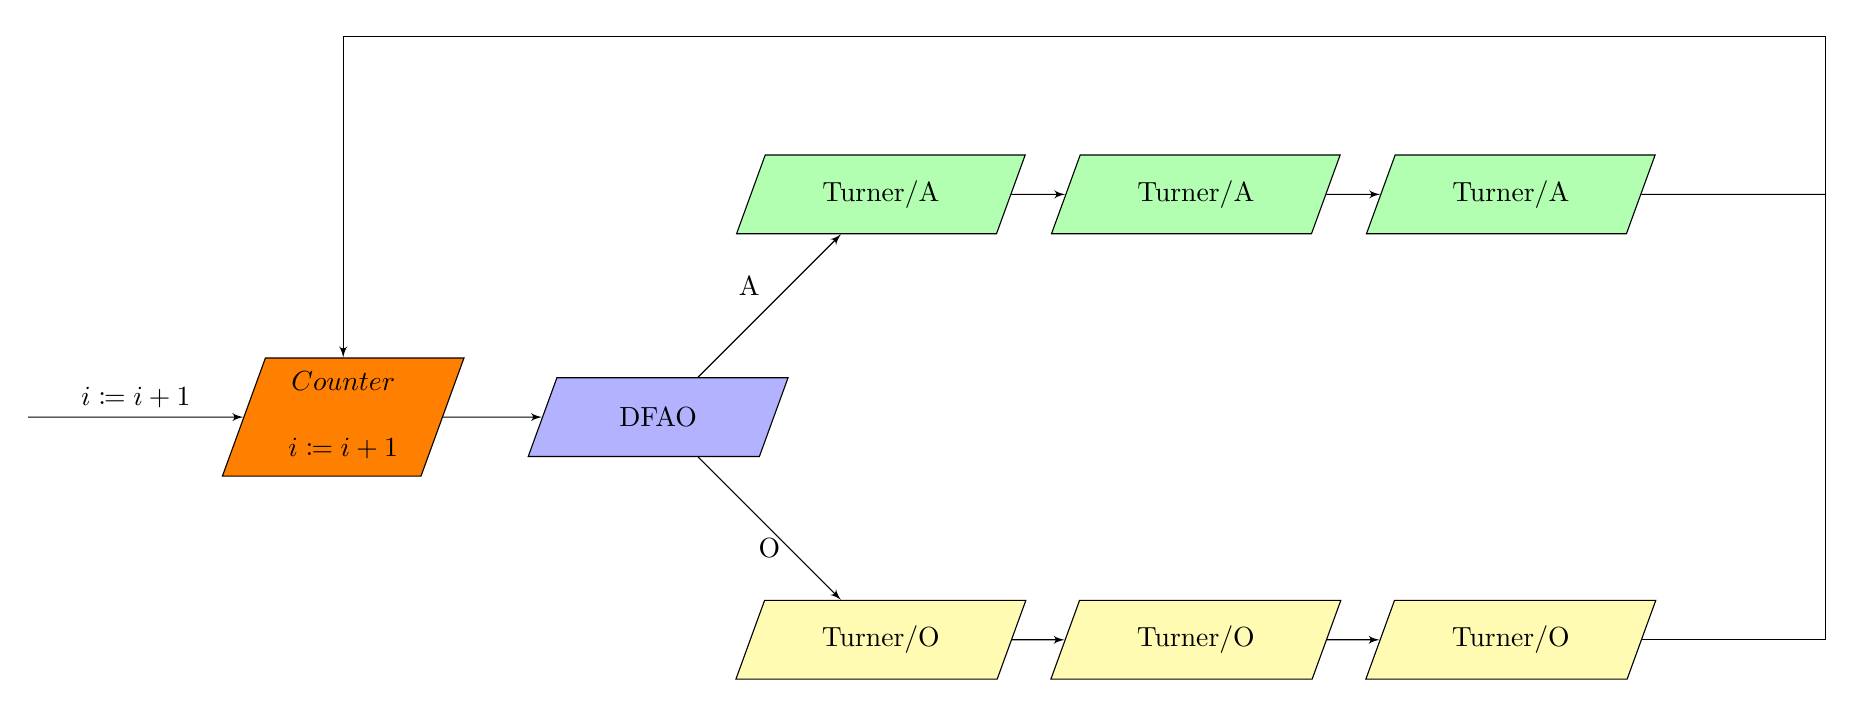
\begin{tikzpicture}[auto, node distance=4cm,>=latex']
\node [input, name=input] {};
\node [block, right of = input , fill=orange] (Counter) {$\begin{array}{cc}Counter\\ \\i\coloneqq i+1 \end{array}$};
\node [block, right of = Counter,  fill=blue!30] (DFAO) {DFAO};
\node [block, above right of = DFAO,  fill =  green!30] (TurnerA) {Turner/A};
\node [block, right of = TurnerA,  fill =  green!30] (TurnerA1) {Turner/A};
\node [block, right of = TurnerA1,  fill =  green!30] (TurnerA2) {Turner/A};
\node [output, name = output, right of =TurnerA2] {};
\node [output, name = output1, above of =output, node distance = 2cm] {};


\node [block, below right of = DFAO,  fill =  yellow!30] (TurnerO) {Turner/O};
\node [block, right of = TurnerO,  fill =  yellow!30] (TurnerO1) {Turner/O};
\node [block, right of = TurnerO1,  fill =  yellow!30] (TurnerO2) {Turner/O};

\draw [draw,->] (input) -- node {$i \coloneqq i + 1$} (Counter);
\draw [draw,->] (Counter) -- node {} (DFAO);
\draw [draw,->] (DFAO) -- node {A} (TurnerA);
\draw [draw,->] (TurnerA) -- node {} (TurnerA1);
\draw [draw,->] (TurnerA1) -- node {} (TurnerA2);

\draw [draw,->,below] (DFAO) -- node {O} (TurnerO);
\draw [draw,->] (TurnerO) -- node {} (TurnerO1);
\draw [draw,->] (TurnerO1) -- node {} (TurnerO2);
\draw [draw,-] (TurnerA2) -- node {} (output);
\draw [draw,-] (output) -- node {} (output1);
\draw [draw,->] (output1) -| node {} (Counter);
\draw [draw,-] (TurnerO2) -| node {} (output);


\end{tikzpicture}
\end{document}